\section{Análise Bivariada}

\subsection{Registros}

\begin{figure}[h!]
\centering
{\scriptsize Tabela 10. Correlação linear entre o número de registros (Log10) por município em cada banco de dados e variáveis explanatórias. WAV = Wikiaves, SLI = SpeciesLink, WAV2 = WAV com municípios redundantes em SLI. Número de municípios (n), coeficiente de correlação de Pearson (r) para cada pareamento, com outliers bivariados excluídos. Valores significantes $(p < 0.05)$ em negrito. }
\\
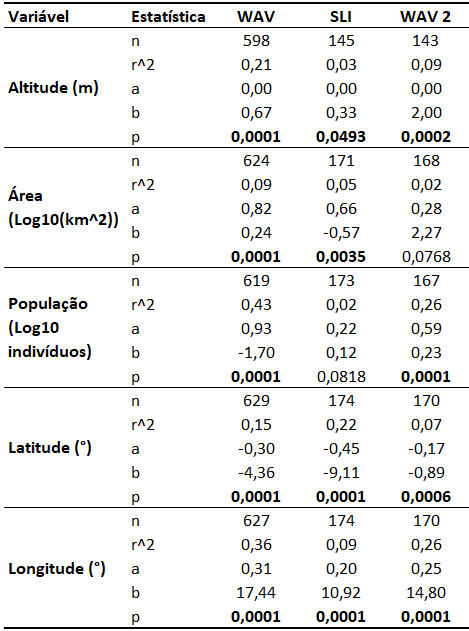
\includegraphics{Tabelas/10.png}
\end{figure}

\texto

\newpage

\subsubsection{Altitude}

\begin{figure}[h!]
\centering
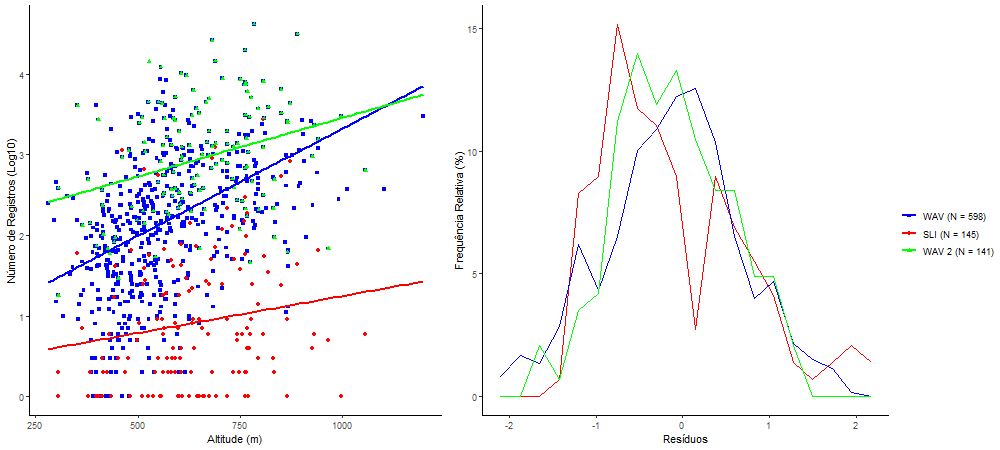
\includegraphics[width = 15cm]{Imagens/31133.png}
\\{\scriptsize Figura 9. Relação linear entre o número de registros (Log10) em cada banco de dados e a altitude (m) da sede dos municípios (esquerda) e respectiva distribuição de resíduos (direita, em unidades de desvio-padrão, em unidades de desvio-padrão). Outliers bivariados foram excluídos. }
\end{figure}


\subsubsection{Área}


\begin{figure}[h!]
\centering
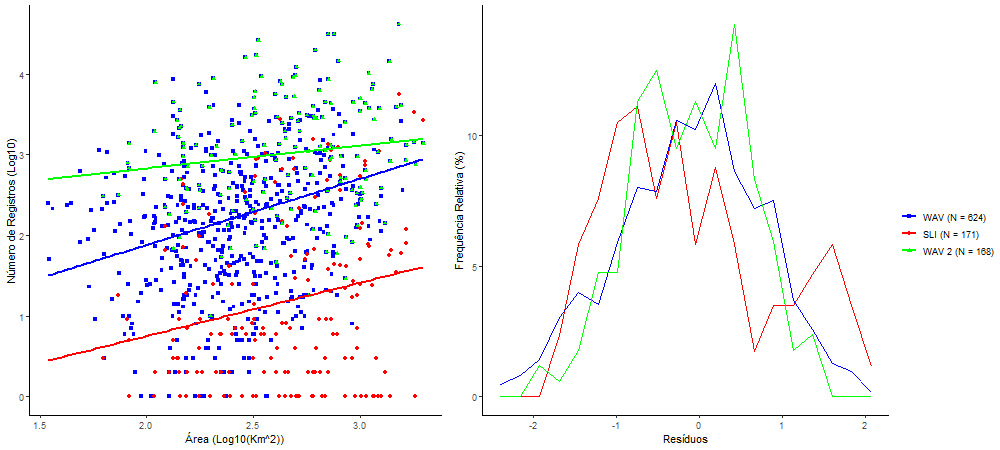
\includegraphics[width = 15cm]{Imagens/31233.png}
\\{\scriptsize Figura 10. Relação linear entre o número de registros (Log10) em cada banco de dados e a área (Log10 km2) dos municípios (esquerda) e respectiva distribuição de resíduos (direita, em unidades de desvio-padrão). Outliers bivariados foram excluídos.}
\end{figure}

\newpage



\subsubsection{População}

\begin{figure}[h!]
\centering
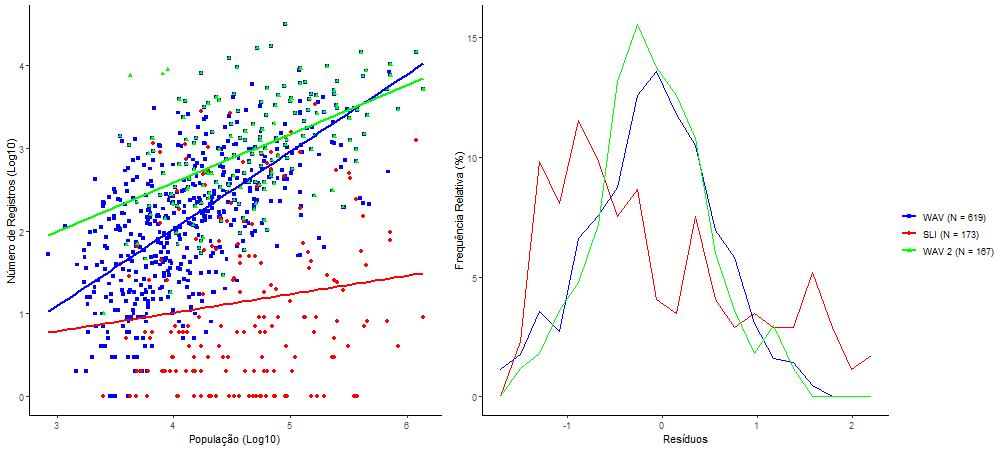
\includegraphics[width = 15cm]{Imagens/31333.png}
\\{\scriptsize Figura 11. Relação linear entre o número de registros (Log10) em cada banco de dados e o tamanho da população humana (Log10 indivíduos) dos municípios (esquerda) e respectiva distribuição de resíduos (direita, em unidades de desvio-padrão). Outliers bivariados foram excluídos.}
\end{figure}


\subsubsection{Latitude}

\begin{figure}[h!]
\centering
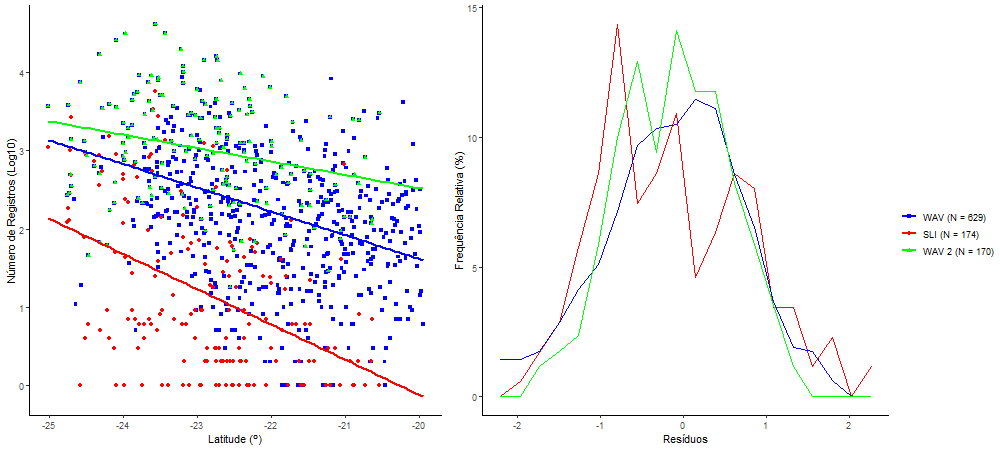
\includegraphics[width = 15cm]{Imagens/31433.png}
\\{\scriptsize Figura 12. Relação linear entre o número de registros (Log10) em cada banco de dados e a latitude (graus) da sede dos municípios (esquerda) e respectiva distribuição de resíduos (direita, em unidades de desvio-padrão). Outliers bivariados foram excluídos.}
\end{figure}

\newpage

\texto

\subsubsection{Longitude}

\begin{figure}[h!]
\centering
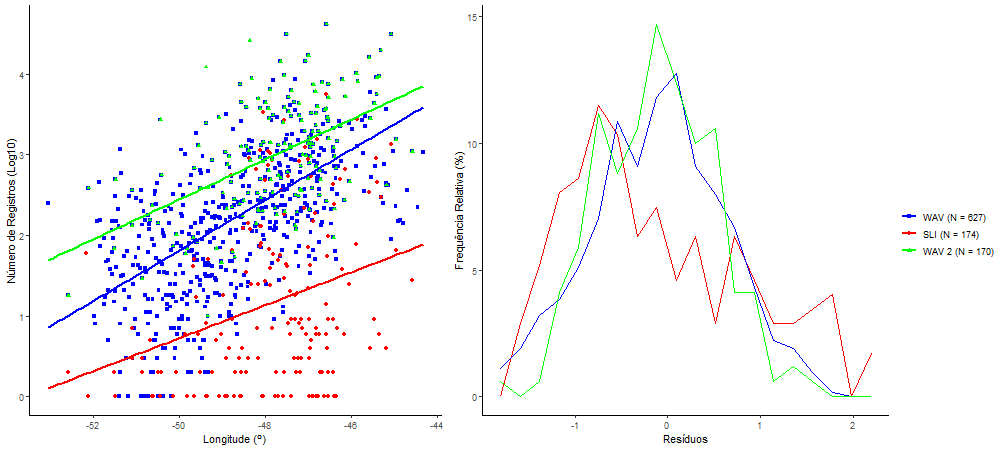
\includegraphics[width = 15cm]{Imagens/31533.png}
\\{\scriptsize Figura 13. Relação linear entre o número de registros (Log10) em cada banco de dados e a longitude (graus) da sede dos municípios (esquerda) e respectiva distribuição de resíduos (direita, em unidades de desvio-padrão). Outliers bivariados foram excluídos.}
\end{figure}

\texto


\subsection{Espécies}

\texto


\begin{figure}[h!]
\centering
{\scriptsize Tabela 11: Correlação linear entre o número de espécies (Log10) por município em cada banco de dados e variáveis explanatórias. WAV = Wikiaves, SLI = SpeciesLink, WAV2 = WAV com municípios redundantes em SLI. Número de municípios (n), coeficiente de correlação de Pearson (r) para cada pareamento, com outliers bivariados excluídos. Valores significantes $(p < 0.05)$ em negrito.}
\\
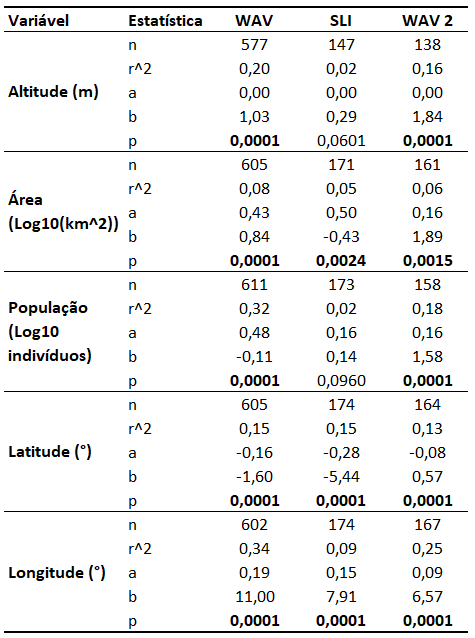
\includegraphics{Tabelas/11.png}
\end{figure}

\subsubsection{Altitude}

\begin{figure}[h!]
\centering
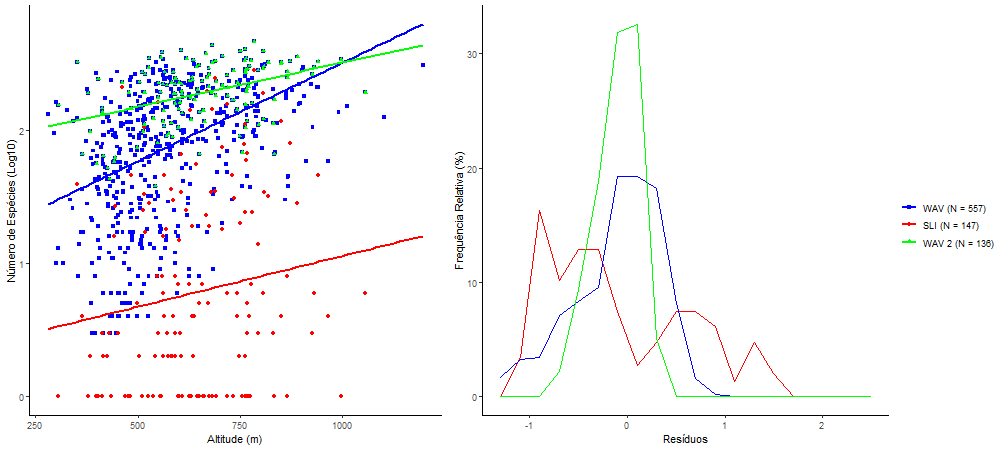
\includegraphics[width = 15cm]{Imagens/32133.png}
\\{\scriptsize Figura 14: Relação linear entre o número de espécies (Log10) em cada banco de dados e a altitude (m) da sede dos municípios (esquerda) e respectiva distribuição de resíduos (direita, em unidades de desvio-padrão). Outliers bivariados foram excluídos.}
\end{figure}


\texto

\subsubsection{Área}



\begin{figure}[h!]
\centering
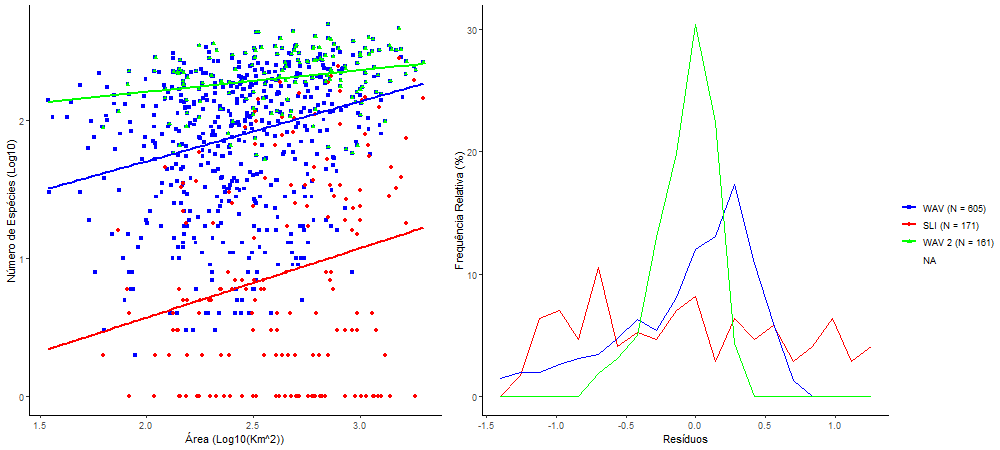
\includegraphics[width = 15cm]{Imagens/32233.png}
\\{\scriptsize Figura 15: Relação linear entre o número de espécies (Log10) em cada banco de dados e a área (Log10 km2) dos municípios (esquerda) e respectiva distribuição de resíduos (direita, em unidades de desvio-padrão). Outliers bivariados foram excluídos.}
\end{figure}

\texto

\subsubsection{População}

\begin{figure}[h!]
\centering
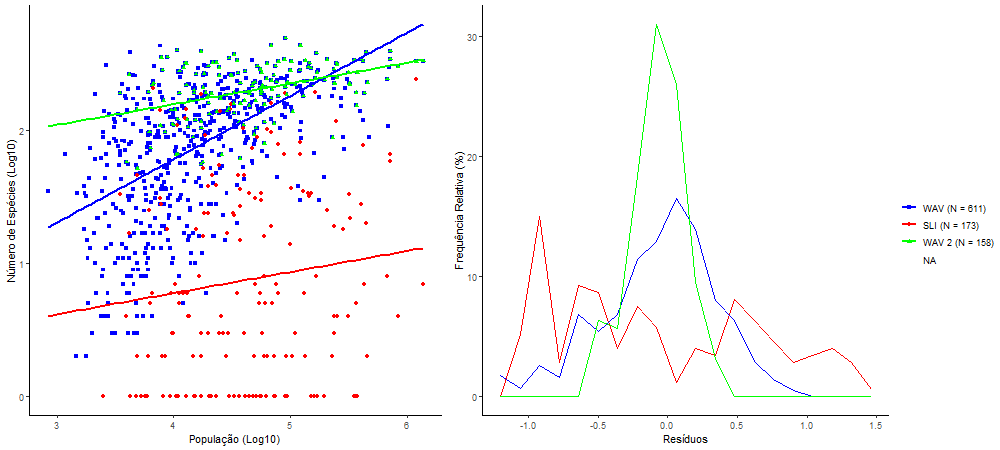
\includegraphics[width = 15cm]{Imagens/32333.png}
\\{\scriptsize Figura 16: Relação linear entre o número de espécies (Log10) em cada banco de dados e o tamanho da população humana (Log10 indivíduos) dos municípios (esquerda) e respectiva distribuição de resíduos (direita, em unidades de desvio-padrão). Outliers bivariados foram excluídos.}
\end{figure}

\texto

\subsubsection{Latitude}

 

\begin{figure}[h!]
\centering
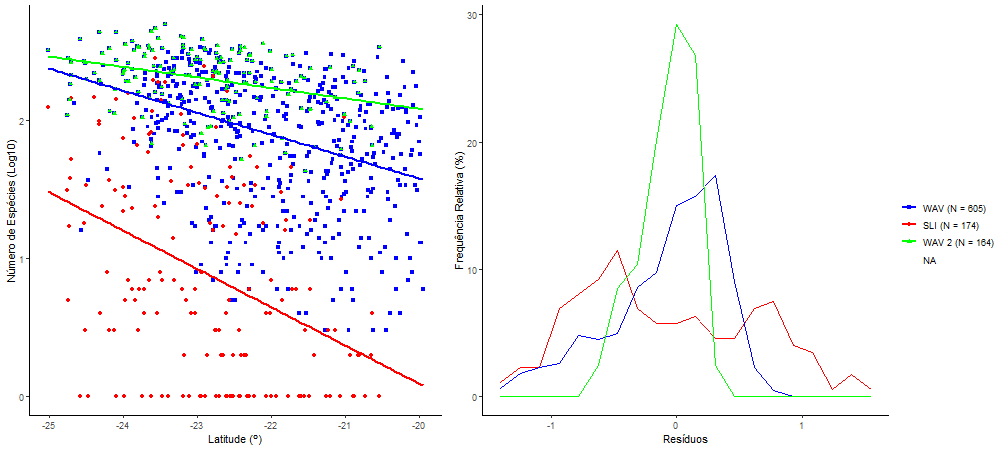
\includegraphics[width = 15cm]{Imagens/32433.png}
\\{\scriptsize Figura 17: Relação linear entre o número de espécies (Log10) em cada banco de dados e a latitude (graus) da sede dos municípios (esquerda) e respectiva distribuição de resíduos (direita, em unidades de desvio-padrão). Outliers bivariados foram excluídos.}
\end{figure}

\texto

\subsubsection{Longitude}

\begin{figure}[h!]
\centering
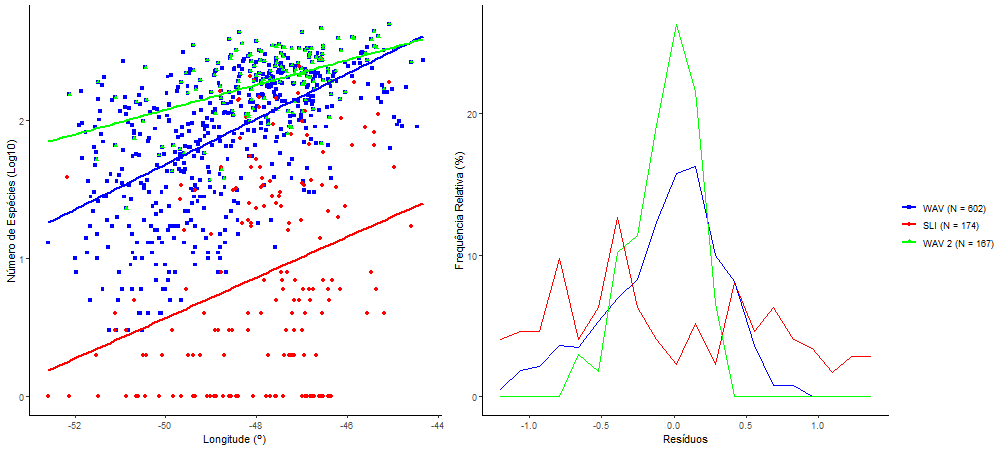
\includegraphics[width = 15cm]{Imagens/32533.png}
\\{\scriptsize Figura 18: Relação linear entre o número de espécies (Log10) em cada banco de dados e a longitude (graus) da sede dos municípios (esquerda) e respectiva distribuição de resíduos (direita, em unidades de desvio-padrão). Outliers bivariados foram excluídos.}
\end{figure}

\texto
